\documentclass[aspectratio=169]{beamer}
\usetheme{Madrid}
\usecolortheme{default}
\usepackage[utf8]{inputenc}
\usepackage[T1]{fontenc}
\usepackage{graphicx}
\usepackage{booktabs}
\usepackage{pgfplots}
\pgfplotsset{compat=1.18}

\graphicspath{{images/}}

\title{Presentation Title}
\subtitle{A Beamer template}
\author{Your Name}
\institute{Your Institution}
\date{\today}

\begin{document}

\begin{frame}
  \titlepage
\end{frame}

\begin{frame}{Outline}
  \tableofcontents
\end{frame}

\section{Introduction}
\begin{frame}{Bullet points with overlays}
  \begin{itemize}
    \item<1-> First point appears immediately
    \item<2-> Second point on the next slide
    \item<3-> Third point after that
  \end{itemize}
\end{frame}

\section{Content}
\begin{frame}{Image and text in columns}
  \begin{columns}[T]
    \begin{column}{0.5\textwidth}
      
\includegraphics[width=\linewidth]{landscape.png}
    \end{column}
    \begin{column}{0.45\textwidth}
      \begin{block}{Observation}
        Images go in the \texttt{images/} folder.
      \end{block}
      \begin{alertblock}{Note}
        Drag \& drop files onto the file tree to upload.
      \end{alertblock}
    \end{column}
  \end{columns}
\end{frame}

\begin{frame}{A plot}
  \centering
  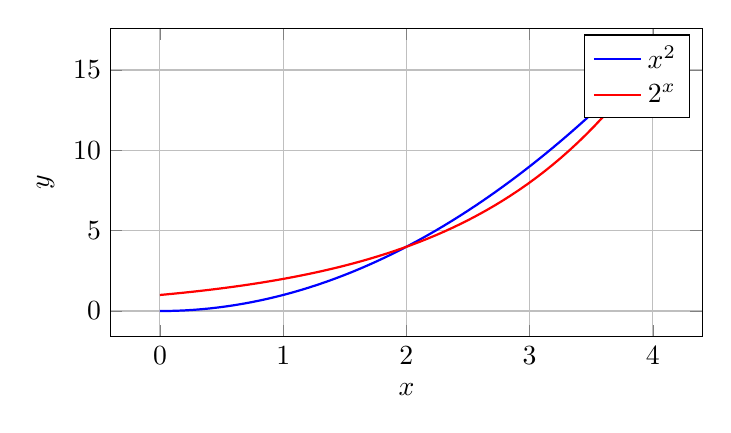
\begin{tikzpicture}
    \begin{axis}[width=0.75\textwidth, height=5.5cm, grid=major, xlabel=$x$, ylabel=$y$, domain=0:4, samples=60]
      \addplot[thick, blue] {x^2};
      \addplot[thick, red] {2^x};
      \legend{$x^2$, $2^x$}
    \end{axis}
  \end{tikzpicture}
\end{frame}

\begin{frame}{A table}
  \centering
  \begin{tabular}{lcc}
    \toprule
    Item & Before & After \\
    \midrule
    Speed & 10 & 25 \\
    Cost  & 100 & 60 \\
    \bottomrule
  \end{tabular}
\end{frame}

\section{Conclusion}
\begin{frame}{Thank you}
  \centering\Large Questions?
\end{frame}

\end{document}
